\documentclass[a4paper,8pt]{article}

% Encoding.
\usepackage{hyperref}
\usepackage{geometry}
\usepackage[T2A]{fontenc}
\usepackage[utf8]{inputenc}
\usepackage[english,russian]{babel}

% Code insertion.
\usepackage[outputdir=build]{minted}

% Math functions.
\usepackage{amsmath}

% Image insertion.
\usepackage{svg}

% No line breaks.
\usepackage[none]{hyphenat}

\title{Задание по курсу ``Администрирование ИС''}
\author{
    \begin{tabular}[t]{c@{\extracolsep{8em}}c} 
        Афанасов Артём     & Смирнов Александр \\
        \\
        Феодор Жилкин    & Филиппов Марк \\
        \\
        Явич Максим
    \end{tabular}
}

\date{\today}

\begin{document}

\maketitle

\tableofcontents

\newpage


\section{Описание ИС}

\subsection{Предметная область}

    \begin{itemize}
        \item Выращивание ЧГ\footnote{Чайный гриб};
        \item Встроенное программирование;
        \item Компьютерное зрение.
    \end{itemize}

\subsection{Цели внедрения ИС}

    \begin{itemize}
        \item Оптимизация обработки заказов;
        \item Масшабирование существующих процессов;
            \begin{itemize}
                \item Выход на новые рынки;
                \item Расширение пользовательской базы;
                \item Масшабирование баз данных;
            \end{itemize}
        \item Анализ накопленных данных по покупкам;
        \item Повышение лояльности пользователей.
    \end{itemize}


\subsection{Преимущества от внедрения ИС}

\subsubsection{Упрощение задач}


    \begin{itemize}
        \item Клиент:
            \begin{itemize}
                \item Поиск ЧГ;
                \item Покупка ЧГ и сопутсвующих товаров;
                \item Уход за ЧГ;
                \item Обращение в службу поддержки по уходу за ЧГ;
            \end{itemize}
        \item Бизнес:
            \begin{itemize}
                \item Обработка заказов;
                \item Анализ приобритаемых товаров;
                \item Масштабируемость нагрузки на приложение;
                \item Оптимизация работы приложения.
            \end{itemize}
    \end{itemize}

\subsubsection{Риски}

    \begin{itemize}
        \item Неактуальный каталог товаров;
        \item Истеречение срока годности;
        \item Потеря клиента на этапе покупки;
        \item Потеря гриба вследствие нарушения правил ухода.
    \end{itemize}

\subsubsection{Безопасность}

    \begin{itemize}
        \item Транзакции при оплате покупок;
        \item Защита датчиков от взлома;
        \item Управление доступом к данным; 
        \item Антивирусная защитa;
        \item Резервное копированиe; 
        \item Информирование об инцидентах в области ИБ.
    \end{itemize}


\subsection{Основные функции}

    \begin{itemize}
        \item Приложение:
            \begin{itemize}
                \item Каталог для продажи ЧГ и аксесcуаров к нему;
                \item Покупка ЧГ;
                \item Отслеживание статуса доставки;
                \item Отслеживание состояния ЧГ по датчикам;
                \item Обращение в службу поддержки;
            \end{itemize}
        \item Датчики:
            \begin{itemize}
                \item Распознавание положения ЧГ в банке;
                \item Температура;
                \item Плотность;
                \item Водородность;
                \item Содержание спирта;
            \end{itemize}
        \item СУБД:
            \begin{itemize}
                \item Хранение информации;
                \item Обработка \& анализ информации;
            \end{itemize}
    \end{itemize}



\subsection{Заинтересованные стороны}

    \begin{itemize}
        \item Заказчик и спонсор проекта:
            \begin{itemize}
                \item ОАО “Eco Slavic Fit”;
            \end{itemize}
        \item Исполнитель:
            \begin{itemize}
                \item ООО “Камбуча-Рус”; 
            \end{itemize}
        \item Ответственные лица:
            \begin{itemize}
                \item Технический руководитель (Жилкин Ф. И.);
                \item Архитектор (Афанасов А. К.);
                \item Системный администратор (Смирнов А. Л.);
                \item Тестировщик (Филиппов Г. Л.);
                \item Старший программист (Явич Х. Ф.).
            \end{itemize}
    \end{itemize}

\section{Разработка ИС}



\subsection{Этапы работ}


    \begin{figure}[h]
        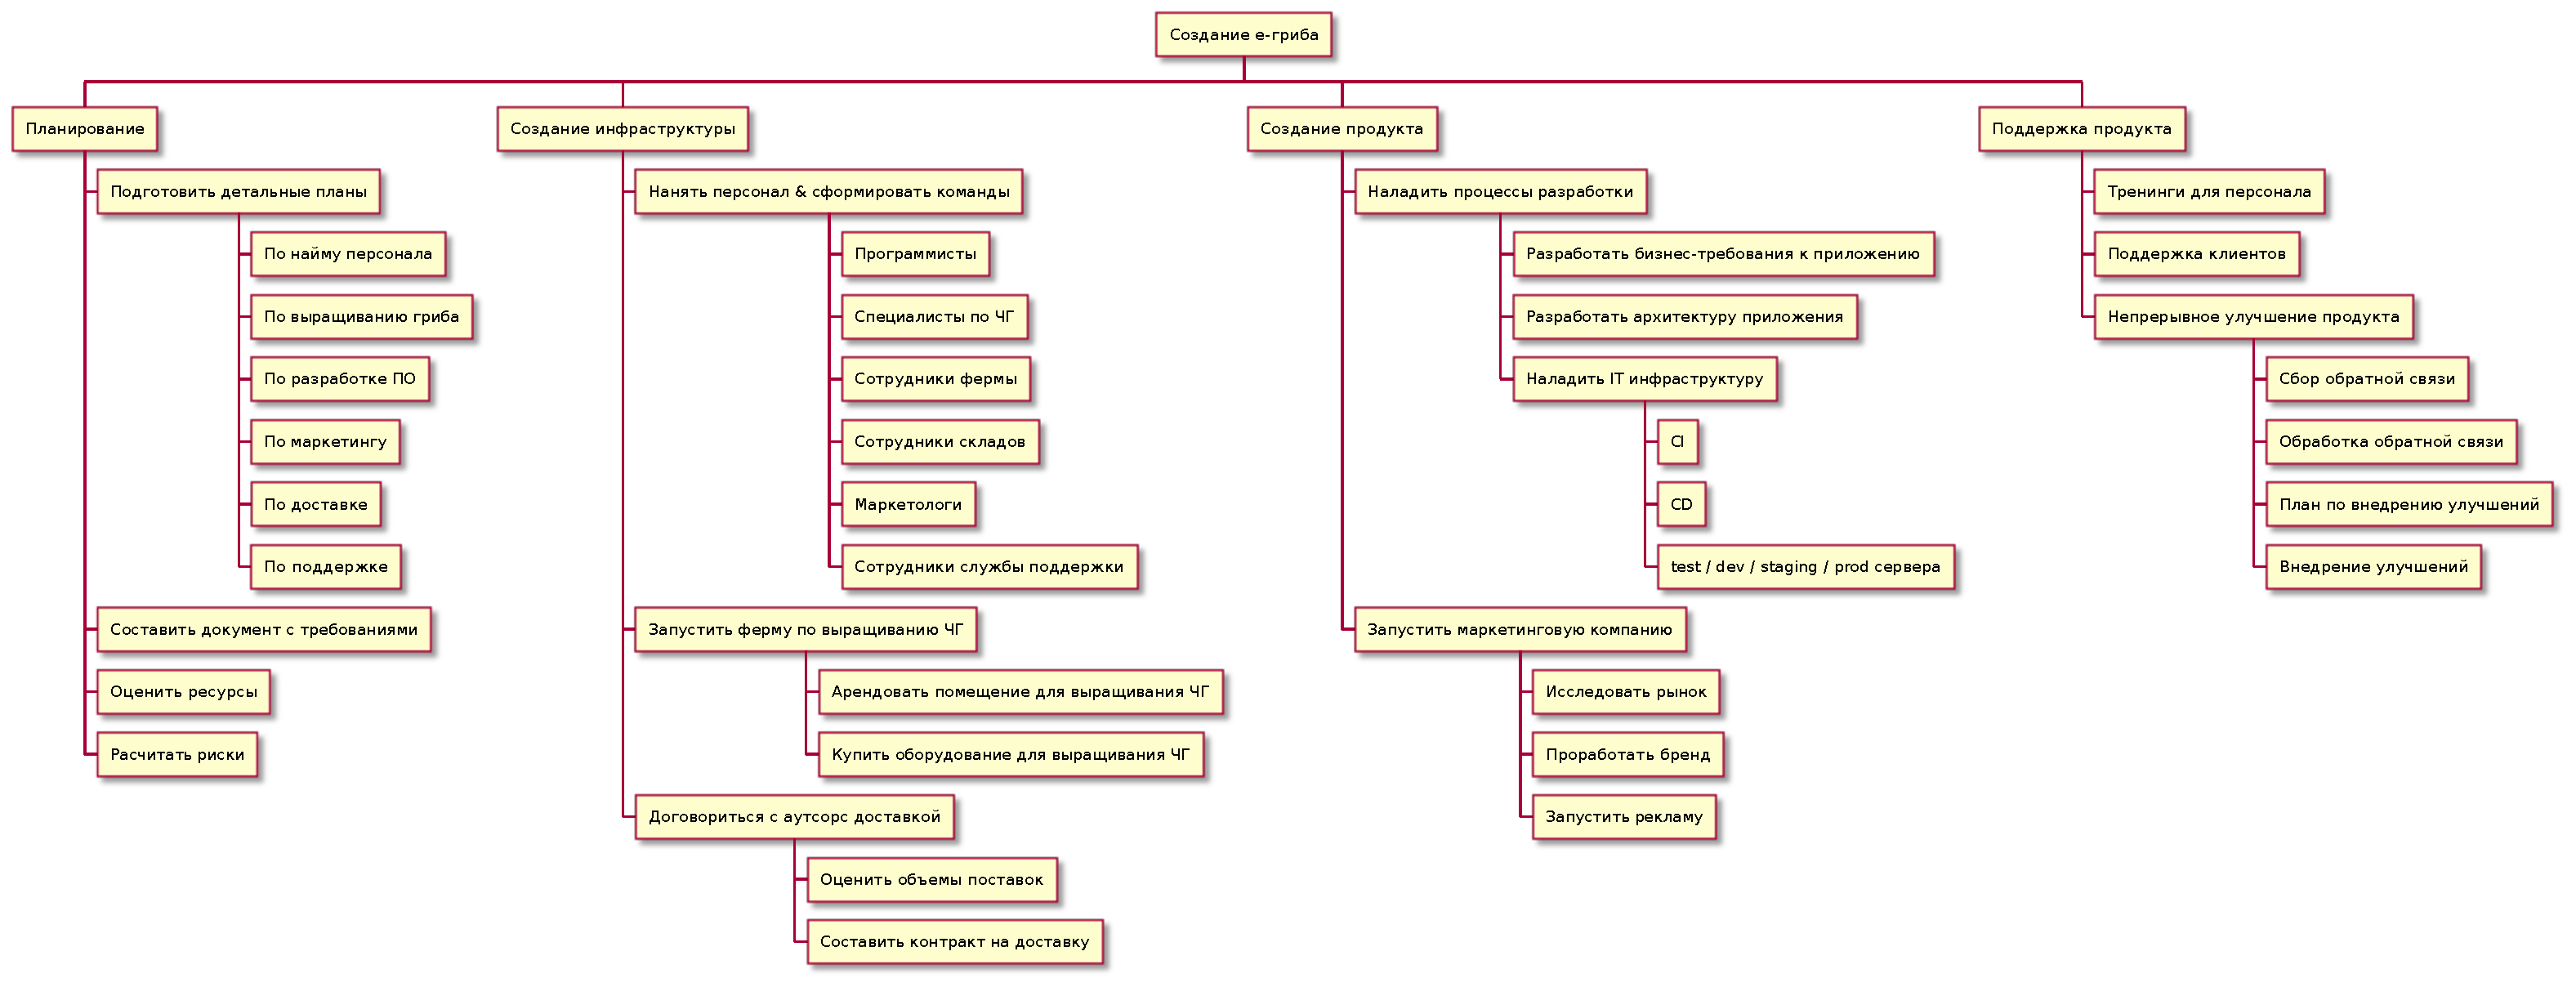
\includegraphics[width=\textwidth]{./pics/wbs.pdf}
        \caption {WBS (можно приближать)}
        \centering

    \end{figure}



\subsection{Риски}

    \begin{itemize}
        \item Кибер атака на систему:
            \begin{itemize}
                \item Периодичность мониторинга -- постоянно;
                \item Реакция -- борьба с вирусом и восстановление данных, работы серверов;
                \item Вероятность -- 5\%;
            \end{itemize}
        \item Потеря базы данных:
            \begin{itemize}
                \item Периодичность мониторинга -- по требованию;
                \item Реакция -- восстановление из резевных копий;
                \item Вероятность -- 10\%;
            \end{itemize}
        \item Дополнительные затраты на поиск сотрудников:
            \begin{itemize}
                \item Периодичность мониторинга -- ежемесячно;
                \item Реакция -- Реклама и Повышение оклада;
                \item Вероятность -- 30-40\%;
            \end{itemize}

        \item Сотрудники не эффективно выполняют свою работу:
            \begin{itemize}
                \item Периодичность мониторинга -- ежедневно;
                \item Реакция -- система поощрения, премии за хорошую работу;
                \item Вероятность -- 10-20\%;
            \end{itemize}

    \end{itemize}



\subsection{Требования}

\subsubsection{Бизнес требования}


    \begin{itemize}
        \item Оптимизация обработки заказов;
        \item Масшабирование существующих процессов;
            \begin{itemize}
                \item Выход на новые рынки;
                \item Расширение пользовательской базы;
                \item Масшабирование баз данных;
            \end{itemize}
        \item Анализ накопленных данных по покупкам;
        \item Повышение лояльности пользователей.
        \item Приложения под платформы:
            \begin{itemize}
                \item iOS;
                \item Android;
            \end{itemize}

    \end{itemize}


\subsubsection{Системные требования}
    \begin{itemize}
        \item iOS:
            \begin{itemize}
                \item iPhone: Требуется iOS 10.0 или новее;
                \item iPad: Требуется iPadOS 10.0 или новее;
                \item iPod touch: Требуется iOS 10.0 или новее;
            \end{itemize}
        \item Android:
            \begin{itemize}
                \item Требуемая версия Andoid: 7 и выше;
                \item От 1 GB оперативной памяти.
            \end{itemize}
    \end{itemize}


\subsubsection{Требования по производительности}

    \begin{itemize}
        \item Приложение должно сохранять высокую отзывчивость при одновременном доступе нескольких пользователей;
        \item Приложение не должно использовать большой объем памяти при небольшом количестве посетителей;
        \item Единственный сервер базы данных должен быстро обслуживать запросы, даже при наличии нескольких серверов приложений, действующих под высокой нагрузкой;
        \item Приложение должно обслуживать каждую страницу не дольше 300 мсек (не включая задержки в сети), при условии одновременного обслуживания не более 5000 пользователей;
        \item Приложение должно потреблять не более 4 Кбайт памяти на каждый неактивный сеанс с пользователем;
        \item Нагрузка на CPU и используемый объем жесткого диска на сервере баз данных не должны превышать 70\%, а время обработки запросов не должно превышать 75 мсек.

    \end{itemize}


\subsubsection{Инфраструктура}

    \begin{itemize}
        \item Процессы CI / CD;
        \item Масштабируемая БД;
        \item Масштабируемые сервера;
        \item Реплики dev / test / staging / prod;
        \item IAAS.
    \end{itemize}


\section{Моделирование}


\subsection{SADT}
\subsection{UML}






\end{document}
